\chapter{肺部粟粒状病灶}

肺部粟粒状(或粟粒样结节)病灶须经X线胸部摄片方能发现。这些细小的弥散性病灶,其直径通常约为1~2mm。许多病变都可产生类似的影像,各种原因的肺部粟粒状病灶常易被误诊为急性、亚急性或慢性粟粒型肺结核,可是粟粒型肺结核较少被误诊为其他原因的粟粒状病灶,肺部粟粒状病灶的疾病分类见表\ref{tab8-1}。对于肺部粟粒状改变的病灶,胸部X线检查是鉴别病变的最重要的评估手段。但是仅靠X线摄片检查往往难于确定诊断,在判断时必须密切结合全面临床材料和其他检查结果。它们在X线上的鉴别要点见表\ref{tab8-2}。

\begin{table}[htbp]
\centering
\caption{肺部粟粒状病灶疾病的分类}
\label{tab8-1}
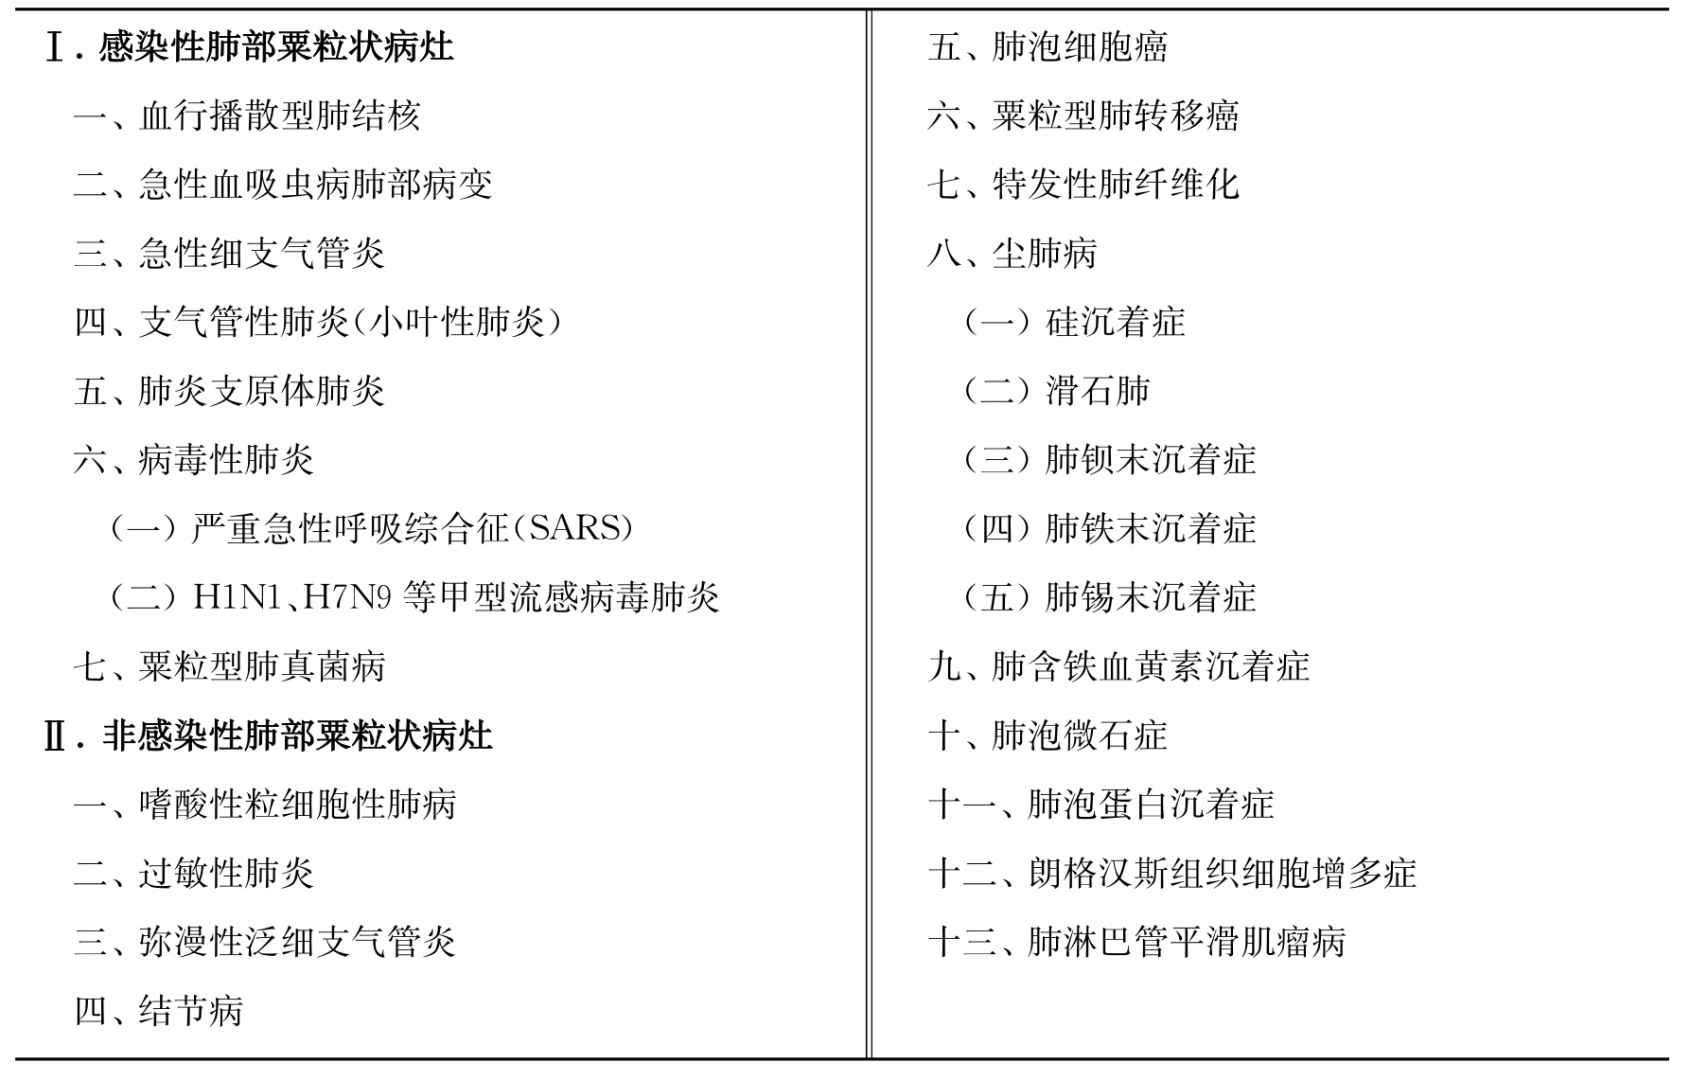
\includegraphics[width=5.94792in,height=3.79167in]{./images/Image00062.jpg}
\end{table}

\begin{table}[htbp]
\centering
\caption{肺部粟粒状病灶在X线胸片上的鉴别要点}
\label{tab8-2}
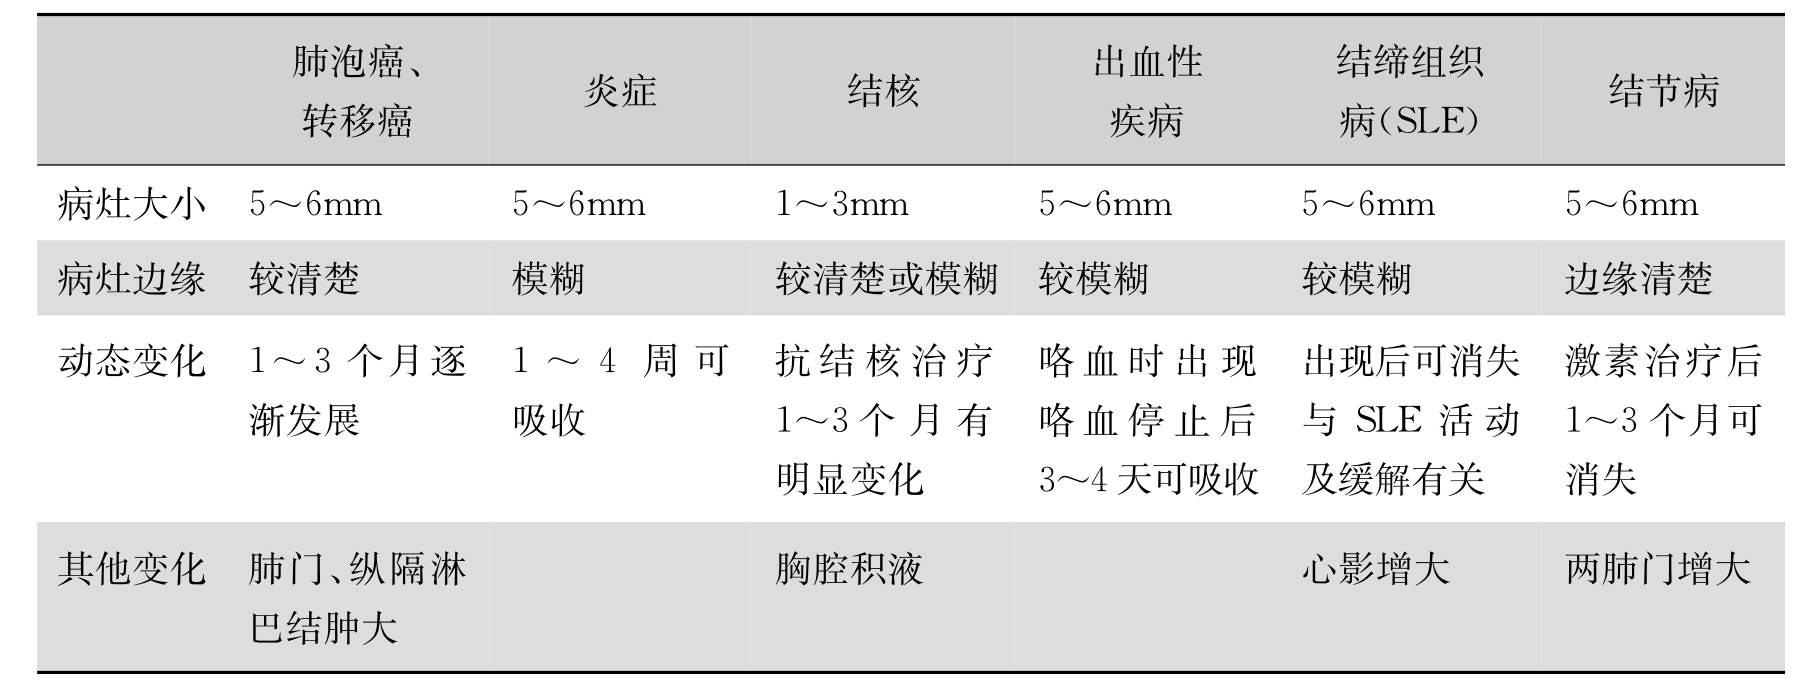
\includegraphics[width=6in,height=2.29167in]{./images/Image00063.jpg}
\end{table}

\protect\hypertarget{text00085.html}{}{}

\section{28 感染性肺部粟粒状病灶}

\subsection{一、血行播散型肺结核}

在各种原因的肺部粟粒状病灶中,以血行播散性肺结核较为多见。血行播散型肺结核的主要特点是肺野内出现广泛分布的粟粒状病灶。按其病程发展的快慢可分为急性、亚急性和慢性血行播散三种类型。

\subsubsection{(一)急性粟粒型肺结核}

由于机体免疫功能降低,超敏反应增高,肺内原发灶及肺门纵隔淋巴结结核内的大量结核菌通过淋巴血行引起血行播散性肺结核乃至全身血行播散性结核病,以儿童、青少年多见。X线透视下全肺呈毛玻璃样,透亮度减低,无法认出粟粒状病灶。X线胸片表现为双肺弥漫性大小、密度基本一致的粟粒状(直径1~3mm)致密阴影,在肺门附近及上、中肺野分布较密,下野较疏。粟粒样小结节影与周围健康肺组织分界较清楚,但如病灶周围有炎性渗出时,其边缘较模糊。患者发病急骤,常伴高热、寒战、全身不适、气促、发绀等菌血症表现及呼吸系统症状。肺部无明显体征,或有细湿啰音,散布双侧肺部。胸部X线改变往往在症状发生后3~4周才能见到。

急性粟粒型肺结核,通常根据X线胸片上或胸部CT上的典型粟粒状结节阴影与临床表现而做出诊断,但有些病例不典型,须结合其他检查方能确定诊断。痰结核菌检查阳性率不高。据报道40\%~80\%病例眼底检查能发现脉络膜结核,有助于血行播散型结核的诊断。经纤维支气管镜取肺组织病理活检和刷片找抗酸杆菌有助于诊断,骨髓穿刺、肝穿刺或血培养,只在必要时行之,如发现粟粒状结核结节或结核菌,对确诊有帮助。

\subsubsection{(二)亚急性与慢性血行播散型肺结核}

由少量结核菌或多次间隔性侵入血液循环所引起。胸片表现为弥散性病灶,呈大小不等、分布不均匀、新旧并存的细小结节状阴影,大多局限于双上肺,有自上肺野逐渐向下蔓延的倾向,或在一侧的肺上部较多。病灶的形态与性质不一,上部有陈旧的纤维钙化灶,而其下则有结节状增殖病灶,有的呈渗出性模糊小点。病情进展时有的病灶互相融合,中间发生崩溃,形成圆形的薄壁小空洞。

亚急性血行播散型肺结核的临床症状较急性粟粒型肺结核轻,但也往往有反复的、间断性慢性结核性中毒症状,如乏力、发热(微热多见)、盗汗、食欲减退、体重减轻、月经不调等;部分病例有咳嗽、咳痰或咯血。慢性血行播散型肺结核多是因患者其他器官患有结核而行胸部检查才发现的。由于其病程经过缓慢,患者全身抵抗力较强,慢性结核性中毒症状较轻或不明显。

体征与病变范围和性质有关。病变轻者无明显肺部体征,或叩诊时呈轻浊音,听诊可听到呼吸音粗糙。如有范围较大的渗出性病灶,常可闻及中、细湿啰音。病灶活动时血沉加快,血象中性粒细胞增多与左移,与病灶活动程度相一致。痰中结核菌的阳性率较急性粟粒型肺结核时高。

\subsection{二、急性血吸虫病肺部病变}

急性血吸虫病的肺部病变较为常见,通常出现于感染后40余天至2个月左右,呼吸道症状大多轻微。除少数呈弥漫性融合病变者有肺实变体征之外,多数病例肺部体征甚少。所见的胸部表现为虫卵引起的嗜酸性脓肿或虫卵结节。在部分急性病例,肺内可出现多数急性虫卵结节,其周围肺泡出现炎性渗出物,X线表现类似肺的粟粒性结核。通常肺的变化甚轻微,一般不导致严重后果。关于肺内虫卵的来源,近年来认为并非成虫寄生在肺内产卵,而主要是通过门-腔静脉之间的交通支而来。在肝内门静脉分支严重阻塞并发门静脉高压的患者,更易发生门-腔静脉交通支的开放。

急性血吸虫病的肺部X线特征如下:

\subsubsection{1.两侧肺纹理增加}

是最早出现的征象,几乎见于所有的病例。

\subsubsection{2.肺野粟粒状阴影}

在发热开始半个月左右,胸片中出现散在性粟粒状阴影,直径约1~3mm,沿肺纹分布,以中、下肺野较为密集。其形状类似急性粟粒型肺结核,但分布不如结核的均匀,数量常不如急性粟粒型肺结核时多,密度较低,边缘略模糊。在病程的高峰(约于发热开始后1~2个月左右)可见如云雾状或雪花状、边缘不清、大小不一的模糊阴影,且有互相融合的倾向。一个月之后可见上述阴影有显著吸收,留下点状、颗粒状或星状阴影,较前缩小,边缘渐变清晰,密度也较高。在以后随诊中阴影逐渐减少,于数月之内大都能吸收消退不留痕迹。

患者血中嗜酸性粒细胞常明显增多,须与热带嗜酸性粒细胞增多症相区别。疫水接触史、血吸虫抗原皮内试验有助于鉴别,如大便毛蚴孵化试验阳性,则诊断更为确实。

\subsection{三、急性细支气管炎}

急性细支气管炎可见于小儿麻疹、百日咳之后,临床上有气促、胸闷、发热、双肺干性与细湿啰音等表现。X线胸片上可见密集的小点状阴影,类似粟粒型肺结核,呈弥漫性不规则分布。小点状阴影较粗糙,边缘模糊,较粟粒型肺结核为大。患儿也无明显的结核中毒症状。肺部阴影的消散较肺炎为慢。此外,可见沿支气管分布有细小淡薄的炎症性改变。

由于结核血行播散在麻疹、百日咳之后较为多见,必须细致鉴别之。如细支气管炎经短期抗菌药物治疗后,病情无明显改善或甚而恶化,须注意继发急性粟粒型肺结核的可能性。对高度怀疑结核播散的病例,应迅速采用诊断性抗结核治疗。

\subsection{四、支气管性肺炎(小叶性肺炎)}

细支气管炎可进一步发展成为支气管性肺炎,其中有一类型的肺部改变呈弥漫性小结节状阴影,大小自粟粒至扁豆大,境界不清,可融合成小叶性或大叶性浸润,肺门阴影模糊增大。此种小结节状阴影与急性粟粒型肺结核不同,后者阴影较圆,大小基本均匀,边缘较清楚,分布也较均匀。

某些病毒性肺炎也可出现两肺多发小结节性影,临床上可有发热症状,也可无任何症状而偶然发现,一般一个月左右可以完全吸收。部分肾移植术后巨细胞病毒性肺炎也可呈双肺多发性5~6mm小结节病灶。应注意鉴别,肾移植后巨细胞病毒性肺炎患者有使用激素和免疫抑制剂病史,外周血白细胞正常或下降,淋巴细胞数下降,以发热、咳嗽、胸闷为主要表现,无痰或少痰。血巨细胞病毒IgM、IgG抗体阳性,巨细胞病毒抗原的DNA、mRNA阳性有助于诊断。

\subsection{五、肺炎支原体肺炎}

有些肺炎支原体肺炎可表现为弥漫性小结节状阴影,酷似急性细支气管炎的粟粒状阴影。小结节状阴影较粗糙而模糊,多呈一侧性分布,以中肺野为多见,常伴有同侧肺门阴影增大与肺纹理增粗(参见第3.1.4节)。

\subsection{六、病毒性肺炎}

由严重急性呼吸综合征(SARS)冠状病毒、呼吸道腺病毒、流感病毒等引起的肺炎,也可表现为双肺弥漫性粟粒样小结节影,针尖大小,伴肺纹理增粗。鉴别诊断主要依靠病原学检查。

\subsubsection{(一)严重急性呼吸综合征(SARS)}

又称传染性非典型性肺炎(AP)。2002年底在我国广东省佛山市发现首例SARS患者,此后在我国北京、山西等地区及东南亚地区相继出现SARS,此病传染性强、潜伏期短、传播快、病情重、病死率高。目前认为其病原体是一种新的冠状病毒,其X线表现可以有五种:①单纯局限型;②局限-广泛型;③多灶型片状及(或)结节状病灶;④间质-实质型;⑤单纯间质型。多灶型SARS的早期表现为肺内多发斑片状及(或)结节状病灶,病灶多较小,密度中等偏淡,轮廓相对较清晰。结合流行病学资料、临床症状、实验室检查、病原学检查、影像学检查有助于本病的诊断和鉴别诊断。

\subsubsection{(二)甲型H1N1流感病毒肺炎}

2009年3月墨西哥暴发“人感染猪流感”疫情,造成人员死亡。研究发现,此次疫情为变异后的新型甲型H1N1流感病毒引起的急性呼吸道传染病,该毒株包含有猪流感、禽流感和人流感三种流感病毒的基因片段,可以通过飞沫、气溶胶、直接接触或间接接触在人间传播。临床主要表现为流感样症状,少数病例病情重,进展迅速,可出现病毒性肺炎,合并呼吸衰竭、多脏器功能损伤,严重者可以导致死亡。胸部X线检查和胸部CT有时表现为双肺弥漫粟粒样阴影,与其他引起双肺粟粒样改变的疾病难以区分,确诊需依靠病原学检查。

本病的诊断主要结合流行病学史、临床表现和病原学检查。病原学检查包括:

\paragraph{(1)病毒核酸检测:}

以RT-PCR法检测呼吸道标本(咽拭子、口腔含漱液、鼻咽或气管抽取物、痰)中的甲型H1N1流感病毒核酸,结果可呈阳性。

\paragraph{(2)病毒分离:}

呼吸道标本中可分离出甲型H1N1流感病毒。合并病毒性肺炎时肺组织中亦可分离出该病毒。

\paragraph{(3)血清学检查:}

动态检测血清甲型H1N1流感病毒特异性中和抗体水平呈4倍或4倍以上升高。

\subsubsection{(三)甲型H7N9流感病毒肺炎}

人感染H7N9禽流感是由H7N9亚型禽流感病毒引起的急性呼吸道传染病。自2013年2月以来,上海市、安徽省、江苏省、浙江省先后发生不明原因重症肺炎病例,其中确诊人感染H7N9禽流感33例,9例死亡。均为散发病例。

患者一般表现为流感样症状,如发热、咳嗽、少痰,可伴有头痛、肌肉酸痛和全身不适。重症患者病情发展迅速,多在5~7天出现重症肺炎,体温大多持续在39℃以上,呼吸困难,可伴有咯血痰;可快速进展为急性呼吸窘迫综合征、脓毒症、感染性休克,甚至多器官功能障碍,部分患者可出现纵隔气肿、胸腔积液等。胸部X线检查和胸部CT有时也表现为双肺弥漫粟粒样阴影,与其他引起双肺粟粒样改变的疾病难以区分,但多数继发细菌感染后表现为单肺或双肺大叶性实变,确诊需依靠病原学检查(方法同甲型H1N1流感病毒肺炎)。

\subsection{七、粟粒型肺真菌病}

肺真菌病的感染方式可有原发性感染和条件性致病两种,其常见的胸部X线表现有斑片状阴影、实变阴影、小结节阴影、空洞阴影。肺白念珠菌病可在肺内形成弥散性粟粒状病灶,其病灶分布以中、下肺野较多,边缘模糊,可互相融合成较大的结节,且双侧肺门淋巴结肿大。如患者长期接受皮质激素与广谱抗生素治疗,肺内出现弥漫性粟粒状病灶,经积极抗结核治疗无效者,须考虑粟粒型肺真菌病的可能性。如痰涂片及(或)培养反复找到曲霉或白念珠菌、血清曲霉和念珠菌特异性抗原阳性等真菌感染证据,纤维支气管镜检查分泌物培养出真菌,或纤支镜病理活检见真菌菌丝和孢子,并经抗真菌治疗后好转,病灶缩小或吸收,则诊断可以确定。

肺粟粒样隐球菌病合并隐球菌性脑膜炎病例亦有报告。

\protect\hypertarget{text00086.html}{}{}

\section{29 非感染性肺部粟粒状病灶}

\subsection{一、嗜酸性粒细胞性肺病}

嗜酸性粒细胞性肺病一般分为不明原因和有特定原因的嗜酸性粒细胞性肺病两类。

不明原因包括:①单纯性肺嗜酸性粒细胞增多症(SPE);②急性嗜酸性粒细胞性肺炎(AEP);③特发性高嗜酸性粒细胞综合征(IHS);④慢性嗜酸性粒细胞性肺炎(CEP)。

特定原因包括:①变应性支气管肺曲霉病(ABPA);②支气管中心性肉芽肿(BG);③寄生虫感染;④药物反应;⑤嗜酸性肉芽肿性多血管炎(Churg-Strauss综合征,CSS)。这类疾病外周血和肺泡灌洗液中嗜酸性粒细胞升高,影像学胸部CT表现为肺部单发或多发实变影、磨玻璃影、网格影、粟粒状小结节影;需结合病史、临床表现、肺组织活检病理检查确定。

\subsubsection{(一)特发性高嗜酸性粒细胞综合征(IHS)}

多发生于20~40岁成年人,病因尚未明确,可能为某种丝虫感染。有的病例在X线胸片上出现弥散性点状阴影,中心密度较大,周围较浅而模糊;少数阴影较大,形成小结节状阴影,类似粟粒型肺结核,但密度与清晰度则不如粟粒型结核。这些点状阴影常呈对称性分布,愈近肺门而愈密,愈靠近周围而愈疏,通常伴肺门阴影增大、肺纹理增加。病灶多以中下肺野为多,肺尖多清晰,只有少数患者可在上肺野有较多的病变。此种病变应与粟粒型肺结核相区别。

本病临床上全身症状较轻,无发热或有微热,典型病例常有阵发性气喘发作。典型病例的诊断主要根据:①长期阵发性咳嗽或哮喘,多半于夜间发作或加剧;②嗜酸性粒细胞计数绝对值增多,致白细胞总数增多;③X线胸片上有肺纹理增加、粟粒样点状阴影、肺门淋巴结肿大等征象。

\subsubsection{(二)慢性嗜酸性粒细胞性肺炎(CEP)}

以外周血嗜酸性粒细胞增高、双肺弥漫性肺间质改变,周边磨玻璃、网格影、粟粒影、肺脏嗜酸性粒细胞浸润为主要特征。肺组织病理示肺间质及肺泡有嗜酸性粒细胞浸润。各年龄组均可发病,平均年龄45岁左右。CEP临床表现无特异性,表现为咳嗽、咳痰、气促、胸闷等呼吸道症状以及发热等全身症状。胸部X线表现为肺部磨玻璃样浸润影,可呈游走性,主要分布在双肺的外周和上肺,特征性表现为“肺水肿反转征”。CEP目前还没有确定的诊断标准,国内外多数专家认为具备以下4项可诊断CEP:①咳嗽及呼吸困难等呼吸道症状持续2周以上;②BALF及(或)外周血嗜酸性粒细胞升高;③胸部影像学检查示周围性肺浸润影;④排除其他原因引起的嗜酸性粒细胞性肺病。肺组织活检结果以嗜酸性粒细胞、巨噬细胞浸润为主的肺泡炎、肺间质纤维化和嗜酸性粒细胞脓肿等病理改变有助于诊断。糖皮质激素治疗有效。本病需与ABPA、CSS、AEP和隐源性机化性肺炎(COP)等鉴别,COP可表现为咳嗽、气促、发热等。一般无哮喘发作症状。肺部多发肺实质和肺间质浸润性阴影可为游走性,抗生素治疗无效,糖皮质激素治疗效果显著。但BALF中淋巴细胞及中性粒细胞比例增多,而非嗜酸性粒细胞增多。肺组织活检病理表现为闭塞性支气管炎伴机化性肺炎。

\subsection{二、过敏性肺炎(HP)}

过敏性肺炎又称外源性过敏性肺泡炎,经典表现为农民肺及鸽子肺。近年来随着工业化发展和生活方式的改变,越来越多的小分子化学物质成为HP新型暴露原。有时X线胸片和CT显示双肺弥漫边界不清的小叶中心性微结节,磨玻璃影,极易误诊为粟粒性肺结核。由于HP临床类型多样化,导致HP诊断困难,目前国际上尚无统一的HP诊断标准,临床误诊、漏诊率高。北京协和医院总结分析了2001~2011年诊断为HP且临床资料完整的96例患者。结果表明,以女性发病为主,中老年人多见,非吸烟者居多;动物蛋白如鸽子、鹦鹉等的羽毛、粪便以及微生物如各类真菌、嗜热放线菌等是HP的暴露因素。工业化越来越多小分子化学物质成为HP一大类新的致敏原。主要临床表现为气短、咳嗽,肺功能检查显示弥散功能障碍及限制性通气功能障碍,嗜酸性粒细胞及IgE均在正常水平,HP属非Ⅰ型变态反应,可通过过敏原特异性IgG抗体检测提示患者接触过暴露原,并不能根据它来诊断HP。HP病理分布呈不均型性、形态多样性,常需与结节病以及感染性肉芽肿性疾病相鉴别。

\subsection{三、弥漫性泛细支气管炎}

弥漫性泛细支气管炎最先在日本报道,近年我国也发现少数病例。本病病因尚未阐明,通常隐袭缓慢发病,常见三大症状为咳嗽、咳痰和活动时气短。双肺听诊断续性湿啰音,以水泡音为主,偶有干啰音及高调喘鸣音。X线胸片是诊断本病的重要依据,典型表现为双肺弥漫散在、边缘不整的颗粒状结节状阴影,直径约2~5mm,以两下肺显著,常伴有肺过度膨胀,有时中叶与舌叶肺不张以及轻、中度支气管扩张。高分辨率CT扫描对本病诊断更有帮助。支气管肺泡灌洗液(BALF)细胞学检查:淋巴细胞、中性粒细胞、嗜酸性粒细胞数增加,T淋巴细胞亚群CD4\textsuperscript{+}
/CD8\textsuperscript{+}
比率降低。纤维支气管镜或胸腔镜下肺组织活检有助于诊断。详细参见第14节。

\subsection{四、结节病}

结节病是一种非干酪性肉芽肿性疾病,可侵犯人体多种器官,以肺和淋巴结为最常受侵器官。结节病约有25\%病例在肺野内出现播散性小斑点状阴影,与急性粟粒型肺结核相似。结节病小结节的大小、形状、密度不同,分布也不均匀,结节在中肺野较上肺野与肺底部为多,且常有两侧肺门淋巴结肿大。患者症状轻微或无明显症状,皮肤病变、浅表淋巴结活检,表现为非干酪性肉芽肿,结合临床及X线表现可作出诊断(参见第26.1节)。

\subsection{五、细支气管肺泡细胞癌}

细支气管肺泡细胞癌多发生在55~65岁之间的老年人,但中青年人发病者也有报道。临床上主要表现为进行性呼吸困难,病史较短,全身中毒症状不明显,多无血丝痰,可有大量的泡沫样黏液痰。肺泡癌的误诊率高,X线胸片上有结节型与弥漫型两种表现,后者胸片表现为双侧肺野弥漫性大小不等的粟粒状病灶,直径1~2mm,在粟粒状结节之间有网状阴影,并于肺下野肋膈角区可见有水平走向胸壁的致密线状影(宽约0.5~1mm,长约2~3cm),外端常抵达胸膜缘(Kerley
B线),可能为淋巴回流受阻的表现,或为癌的直接浸润所致。一般认为此种粟粒状病灶密度中等,边缘模糊,易趋融合,分布以双肺中、下野及内中带较多,双肺上野(特别是肺尖部)甚少,是肺泡癌比较特别的X线征象。这种征象也与粟粒型肺结核有别。结合患者的病情进展较慢、全身中毒症状不明显、大量泡沫样黏液痰等表现,应考虑肺泡癌的可能性。痰中癌细胞阳性可确定诊断(参见第16节)。

有下列表现:①患者在35岁以上,忽然发现双侧中、下野结节状或点片状阴影者;②患者发热、气短与胸片表现不相称,尤其是呼吸困难呈进行性加重者;③经正规抗结核治疗不见好转者,应注意细支气管肺泡癌的可能。

\subsection{六、粟粒型肺转移癌}

肺内转移癌常见,但形成粟粒型转移癌者少见。国内文献有少数病例报告,原发癌部位在胃。临床上也见有肝癌的粟粒型肺转移。粟粒型转移癌易被误诊为血行播散型肺结核。因大量癌细胞广泛转移,引起两肺广泛性小点状阴影,与血行播散型肺结核相似,但其结节较粟粒型结核为大(直径4~8mm),且有增大的倾向,密度也较高,边缘不整齐,大小分布不如粟粒型肺结核均匀。肺门纵隔淋巴结也常增大,并常出现Kerley线。此线主要有A、B两种。B线上文已有述及。A线则是从肺野外围放射状引向肺门的(长约5~6cm,宽约0.5~1mm)线状阴影,它不分支,也不与支气管及血管的走行一致。肺内粟粒型转移癌的诊断,主要根据是发现原发癌的存在,或患者曾有癌病史,经过治疗(如手术切除)而暂被认为“临床治愈”者。

\subsection{七、特发性肺纤维化}

此病的典型症状是进行性气促、咳嗽与咳痰。急性型早期即出现气促,病情迅速恶化,因缺氧与急性右心衰竭而死亡。慢性型起病缓慢,出现咳嗽、咳痰、气短等症状,并呈进行性加重,晚期出现杵状指与慢性肺源性心脏病。典型的X线征为肺野弥漫性条索状或交错的肺纹理增粗增多,可蔓延及外周。急性型可表现为支气管肺炎或慢性肺炎的片状阴影。慢性型胸片上可出现弥漫性较粗糙的粟粒状结节阴影。国内曾有一例被误诊为亚急性血行播散型肺结核,经开胸探查活检确定诊断(参见第15节)。

\subsection{八、尘肺病}

\subsubsection{(一)硅沉着症}

Ⅱ期硅沉着症表现为胸片上肺野出现弥漫性小结节,多分布于肺中、下野。小结节直径1~2mm,边缘一般清晰,往往同时伴有肺门阴影增大、肺纹理增强及肺气肿等表现。Ⅱ期硅沉着症须与急性粟粒型肺结核相区别。但硅沉着症与肺结核并存者并不少见(参见第15节)。

急性粟粒型肺结核的中毒症状明显,痰结核菌可呈阳性,肺门阴影不如硅沉着症的明显增大,点状阴影之间并无肺气肿征象。此外下列四项在鉴别诊断上可供参考:①Ⅱ期硅沉着症的胸片上,部分肺野可见到增多而变粗的肺纹阴影或网织状阴影;②粟粒型肺结核病灶的大小、形态、密度、分布几相等,比硅沉着症更为明显,近乎“绝对相等”;③粟粒型肺结核阴影的密度一般较硅沉着症结节阴影略淡,中心与边缘密度相等;④有人曾报告半数硅沉着症病例的膈肌与纵隔的形态不规则。

在X线胸片上,上述各点对鉴别Ⅱ期硅沉着症与急性粟粒型肺结核有帮助。可是,临床医生不应单凭X线胸片所见而作出诊断,必须对患者作全面的检查。硅沉着症患者有较长工龄的职业接触史,而持久不退的高热与眼底检查所见均有助于粟粒型肺结核的诊断。对于一个可能发生硅沉着症的工人,如突然发生高热,而胸片上X线征象难以区别硅沉着症或粟粒型肺结核时,应考虑作积极的抗结核治疗,从药物疗效来证实或排除粟粒型肺结核的诊断。

\subsubsection{(二)滑石肺}

长期的滑石粉尘接触史提示滑石肺的重要诊断根据。滑石肺的X线征是:肺纹理增多、增深、变粗,并形成大小约2mm(很少达到4mm以上)的小结节状阴影,散布于两肺,尤以两下肺野较多。

\subsubsection{(三)肺钡末沉着症}

此病是重晶石矿或硫酸钡工厂作业工人,长期吸入硫酸钡粉尘所引起的职业病。临床症状一般不明显,远比硅沉着症或矽酸盐肺轻微,大部分无任何主诉。

X线胸片所见为双侧肺野出现弥漫性、细小的深白色斑点状阴影,直径多在1~2mm左右,很少超过3mm,边缘清楚,形状不规则。小结节高度致密,增长缓慢而无融合的倾向,在全肺野同时出现,故与矽肺有所不同。

\subsubsection{(四)肺铁末沉着症}

肺铁末沉着症是产业工人职业病,患者多为电焊工与磨针工。工龄一般在10年以上。患者的临床症状多不明显,虽X线表现肺部病变较重,而肺功能正常或轻度损害,半数以上有不定时的气闷感。肺部体检无异常发现。本症属于良性尘肺。X线胸片检查可见:①大小几乎相等的小结节状圆形或椭圆形的阴影,直径在1~3mm左右,比较均匀而对称散布于两肺野(中、下野较多,肺尖最少);②粟粒状病灶密度不甚高,边缘清楚,无融合的倾向;③肺门改变轻微,或无改变;④两肺纹理呈网状,但纤维增生现象不明显;⑤很少合并肺气肿或胸膜改变。以上各点均有助于与矽肺相区别。在X线胸片上肺铁末沉着症与矽肺虽有些区别,但并无绝对意义。铁末沉着症与其他尘肺的鉴别,职业史甚为重要。

\subsubsection{(五)肺锡末沉着症}

肺锡末沉着症(锡尘肺)是炼锡工人在冶炼过程中,长期吸入含有二氧化锡的气溶胶而产生的肺部疾病,罹患工龄自6~32年不等。患者症状较轻,可有胸闷及轻度胸痛、咳嗽、咳痰等症状。体检胸部一般无明显体征,个别可听到呼吸音粗糙及间断的干性啰音。病情远较硅沉着症为轻,并发肺结核的患病率也不高。

本症的X线胸片有特殊的征象,主要表现为:①肺门一般不增大,但密度异常增高;②两肺野均匀散布的弥漫性点状阴影,一般以中、下野较为密集;点状阴影直径1~2mm,密度高,形状多种多样,大多中心致密,边缘不整,但清楚;③肺纹理增多,肺底透亮度增高;颇似早期代偿性肺气肿;④胸膜和心脏改变不明显。肺功能一般良好,胸廓无改变。诊断须根据长期的锡粉尘接触史与X线胸片所见,并除外其他原因的尘肺,尤其是硅沉着症而确定之。

\subsection{九、肺含铁血黄素沉着症}

肺含铁血黄素沉着症通常继发于风湿性二尖瓣膜病的病程中,因肺循环长期淤血引起,临床上少见;也有特发性者。在X线胸片上可见双肺野有广泛散布的、大小均等的点状密影,自针头大至直径2~3mm,以双侧中、下肺肺门周围较为密集,肺尖部较清晰。继发性病例有心脏增大与外形的改变。本症的特点是胸片点状阴影长期存在而无改变,临床上无结核中毒症状,血中无嗜酸性粒细胞增多,也无尘肺职业史,而有别于粟粒型肺结核、急性血吸虫病及各类型尘肺。患者症状有气短、咳嗽、咳痰、咯血痰、肺底湿啰音等。痰涂片检查见大量含铁血黄素颗粒的吞噬细胞,符合肺含铁血黄素沉着症。

\subsection{十、肺泡微石症}

肺泡微石症是一种原因未明的肺部疾病,可有家族史。患者无尘肺职业史,长期经过无明显症状。后期往往出现咳嗽、咳痰、气短、胸闷,并可出现右心室增大等症状,痰中可混有“鱼子”样小矽粒,胸部听诊可发现双肺呼吸音减弱。X线胸片上可见双肺有弥漫性“鱼子”(鱼卵)样细小钙化胡影,大小相近,边缘清楚,密度较高,以内侧及肺下野较为密集。此种细小粒状阴影可互相融合。但肺门大小正常,未见淋巴结肿大。实验室检查无特殊发现。

本病的诊断主要根据:①经X线检查而发现,多年经过无明显症状;②体格检查与化验检查无明显异常;③可有家族病史而无尘肺职业史;④有上述的特殊X线征;⑤长期随诊X线胸片阴影改变不大。本病易与粟粒型肺结核、肺真菌病及其他尘肺相混淆,主要根据上述的表现而鉴别(表\ref{tab8-3})。

\begin{table}[htbp]
\centering
\caption{肺泡微石症、粟粒性肺结核与硅沉着症的鉴别}
\label{tab8-3}
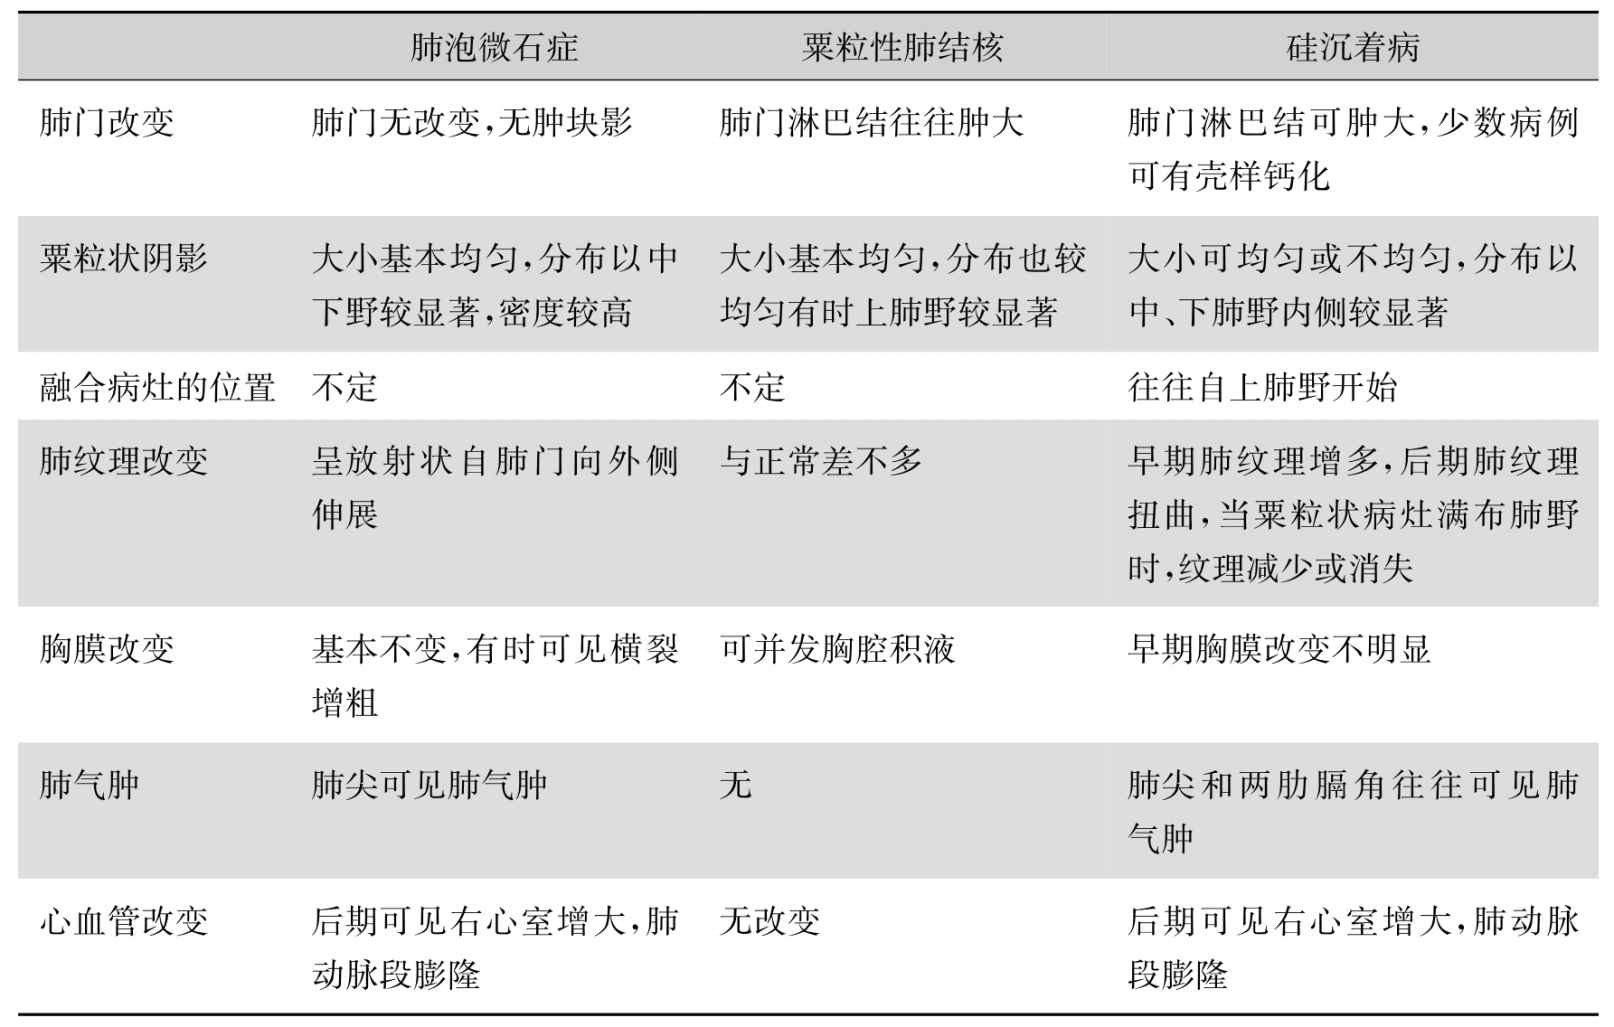
\includegraphics[width=5.9375in,height=3.78125in]{./images/Image00064.jpg}
\end{table}

\subsection{十一、肺泡蛋白沉积症}

肺泡蛋白沉积症也是一种病因不明的疾病,其特征是肺泡和细支气管腔内充满无形态的、过碘酸雪夫(PAS)染色阳性的富磷脂物质。肺泡无炎症表现和极少纤维化,肺泡壁及其间质在病理上无异常改变。主要表现为肺泡内气体交换紊乱,休息状态下患者可出现胸闷、低氧血症,并随运动而加剧。主要死亡原因是低氧血症。

本病典型的X线表现为地图征或铺路石征,也可显示为散在的粟粒状或颗粒状密度增高影,轮廓不很清楚。病变广泛对称或不对称地分布于两肺,不少病例病变分布以中央部位为较多,自肺门向外周放射,形成蝶翼状影,类似肺泡性肺水肿。与肺水肿不同点为本病一般无心脏扩大、肺淤血和间质性肺水肿征象。通常无肺门淋巴结肿大或胸腔积液,病变无钙化征象。肺泡蛋白沉着症的肺部实变、阴影可以存在数月至数年,发现肺部大量实变阴影而临床症状很少者,应考虑本病的可能。

支气管肺泡灌洗液、肺活检、痰液检出PAS染色阳性的脂质有助于诊断。纤支镜肺组织活检在电子显微镜下可见肺泡巨噬细胞包涵体。包涵体周缘有薄膜包绕,内含嗜锇颗粒或板层体。

大容量肺泡灌洗对治疗肺泡蛋白沉着症的疗效确切。

\subsection{十二、肺朗格汉斯细胞组织细胞增多症}

本病原称组织细胞增多症X,病因不明,趋向于侵犯多种组织器官,肺是最常受累的器官(85\%以上),可发生于任何年龄。约25\%的患者无临床症状,仅在做X线检查时发现。常见症状是干咳(56\%~70\%)、呼吸困难(40\%)、胸痛(10\%~20\%)、乏力(30\%)或发热(15\%)。约25\%的患者可发生反复发作的气胸。4\%~20\%的患者可有骨骼的囊性病变。可出现继发性肺动脉高压,晚期可以进展为肺源性心脏病。

在X线胸片和CT上,肺部侵犯表现为两肺广泛和对称性的间质细小结节影和囊腔。结节直径为1~2mm大小,密度淡而模糊。结节病变可吸收,如不吸收则发展为间质性纤维病变,表现为两肺广泛的结节病变和网状纤维病变同时存在,最后可发展为两肺广泛性的网状纤维病,伴有广泛的小泡性肺气肿和囊性病变呈蜂窝状肺。

\subsection{十三、肺淋巴管平滑肌瘤病}

肺淋巴管平滑肌瘤病(lymphangioleiomyomatosis,LAM)是一种罕见的、发病机制尚不清楚的弥漫性肺部疾病,常见于育龄期妇女。该病以异常的平滑肌细胞在气道、淋巴管及血管等中异常增殖为特点,最终导致肺实质形成薄壁囊状结构,导致肺功能减退。肺淋巴管平滑肌瘤病最常见症状为活动后呼吸困难、反复发作自发性气胸、咯血,其他还包括咳嗽、胸痛、乳糜胸(腹)腔积液、乏力等,其中有50\%以上病例以自发性气胸为首发症状。早期胸片可无异常改变或仅有肺纹理增多,病情进展可表现为两肺弥漫性网状、网结节影或粟粒状影,分布较均匀。后期见蜂窝状、囊状改变。高分辨率CT为本病最具诊断价值的影像学检查,表现为弥漫性分布的类圆形薄壁囊状阴影,囊腔直径以2~5mm为主,可见6~30mm的大囊腔,囊腔面积和形态与疾病的严重程度有关。与黑色素瘤相关的HMB45抗体阳性为淋巴管平滑肌瘤病的标记性抗体。确诊有赖于病理学检查。

\protect\hypertarget{text00087.html}{}{}

\section{参考文献}

1.雷建平.125例粟粒型肺结核诊断问题分析.中华结核和呼吸杂志,1990,13:214

2.李龙芸,等.血行播散型肺结核182例临床分析.中华内科杂志,1998,37(12):797

3.黎磊石.热带嗜酸细胞增多症与蠕虫病.中华内科杂志,1963,11:553

4.周新张.热带性肺嗜酸粒细胞增多症.中国实用内科杂志,2002,22(6):324

5.许广润,等.细支气管-肺泡癌24例临床分析.中华内科杂志,1980,19(6):403

6.李荣锦.细支气管肺泡癌(综述).中华结核和呼吸系统疾病杂志,1981,4(1):55

7.肖长生.成人肺部弥漫性、粟粒、斑点状阴影诊断问题的探讨.中华结核和呼吸系统疾病杂志,1984,7:74

8.王保宏,等.多结节型细支气管肺泡癌影像诊断及误诊.实用放射学杂志,2004,20(30):230

9.曹来宾,等.肺钡末沉着症.中华放射学杂志,1965,10:108

10.王之桐,等.焊接工人尘肺.中华内科杂志,1959,7:672

11.北京医学院第三附属医院.电焊工尘肺五例报告.中华医学杂志,1975,55:583

12.广东省职业病防治院.锡末沉着症及用二巯基丙磺酸钠治疗的观察.中华医学杂志,1974,54:435

13.汤鼎铭,等.特发性肺含铁血黄素沉着症5例报告.新医学,1976,7(6):278

14.薛婉芬.特发性含铁血黄素沉着症一例.中华结核和呼吸系统疾病杂志,1986,9:337

15.章鸿靖,等.家族性肺泡微石症.中华放射学杂志,1965,10:239

16.邹恒诰,等.家族性肺泡微石症(附两个家族4例报告).中华放射学杂志,1978,12:126

17.史志澄.职业性肺病.中华结核和呼吸系统疾病杂志,1986,9:54

18.金美玲,等.肺淋巴管平滑肌瘤病.中华结核和呼吸杂志,2000,23:355

19.张晓彤,等.27例血行播散型结核病临床分析.中华内科杂志,2004,43(1)41-44

20.马玙.浅谈血行播散型肺结核的诊断.中华内科杂志,1998,37(12):795

21.肖正伦,等.78例重症急性呼吸综合征病例临床分析.中华结核和呼吸杂志,2003,26(6):334-338

22.张德平.嗜酸性粒细胞性肺病:亟待澄清认识.中华结核和呼吸杂志,2011,34(7):537-539

23.金贝贝,等.过敏性肺炎96例临床特征分析.中华结核和呼吸杂志,2013,36(2):83-87

24.官新立,等.肺泡蛋白沉着症的影像学表现及鉴别诊断.中华全科医学,2010,8(3):374-376

25.王保宏,等.多结节型细支气管肺泡癌影像诊断及误诊实用放射学杂志,2004,20(30):230-233

26.美国胸科学会,欧洲呼吸学会,日本呼吸学会等.特发性肺纤维化诊治循证指南(摘译本).中华结核和呼吸杂志,2011,34(7):486-494.

27.李清泉,杨炯.肺脏疾病鉴别诊断学.北京:科学出版社,2003,279-298

28.朱元珏,陈文彬.呼吸病学.北京:人民卫生出版社,2003,1097,1173,1356-1360

29.卢韶华,等.肺淋巴管肌瘤病的临床及病理特点.中华结核和呼吸杂志,2009,32(9):,664-669

\protect\hypertarget{text00088.html}{}{}

